\subsubsection{Definition}
Christian Goldbach hat als wahrscheinlich erster vermutet, dass jede gerade Zahl, die groesser als 2 ist, als Summe von zwei Primzahlen dargestellt werden kann. Dies ist die Starke Goldbachsche Vermutung. Aus dieser Starken Vermutung geht die Schwache Goldbachsche Vermutung hervor, welchehingegen aussagt, dass jede ungerade Zahl, welche groesser als 5 ist, als Summe von 3 Primzahlen dargestellt werden kann. Bis heute gibt es keinen Beweis fuer die Goldbachsche Vermutung, verschiedene Computerberechnungen zeigen jedoch, dass die Vermutung  bis Zahlengroessen bis zu $4\cdot10^{18}$ zutrifft. Auch die Moeglichkeiten, gerade Zahlen groesser als 2 als Summe zweier Primzahlen darzustellen, steigt, je groesser die gerade Zahl ist. Es laesst sich also vermuten, dass die Vermutung wahr ist, bewiesen ist sie dadurch jedoch nicht. Der deutsche Mathemathiker David Hilbert nach die Starke Goldbachsche Vermutung als sein achtes Problem in seine Liste "Hilbertsche Probleme" auf.
\subsubsection{Starke Goldbachsche Vermutung}
Die Starke Goldbachsche Vermutung, oder auch Binaere Goldbachsche Vermutung genannt, besagt, dass jede gerade Zahl $n$, die groesser als 2 ist, als Summe zweier Primzahlen abgebildet werden kann. Also $n = p + q$, wobei $p$ und $q$ die beiden Primzahlen sind. Generell ist die Darstellung von $n$ nicht eindeutig. $n$ kann in den meisten Faellen als Summe verschiedener Primzahlpaare dargestellt werden.
\subsubsection{Schwache Goldbachsche Vermutung}
Die Schwache Goldbachsche Vermutung, oder Ternaere Goldbachsche Vermutung, geht aus der Starken Goldbachschen Vermutung hervor. Sie besagt, dass ungerade Zahlen $u$, die groesser als $5$ sind, als Summe dreier Primzahlen dargestellt werden kann: $u = p + q + r$. Ist der Umstand gegeben, dass die Starke Goldbachsche Vermutung wahr ist, so ist $u = (u - 3) + 3$. $u - 3$ ist hierbei nach Goldbach die Summe zweier Primzahlen, also $u - 3 = p + q$. Somit ist die Darstellung von $u$ als Summe von 3 Primzahlen gegeben: $u = p + q + 3$. Wie bei der Starken Vermutung ist die Abbildung nicht eindeutig. $u$ kann also, mit Ausnahme von der Primzahl $7$, durch unterschiedliche Summanden abgebildet werden.
\subsubsection{Finden von Summendarstellungen}
Das Finden von Summendarstellungen basiert auf dem Sieb des Eratosthenes, welches zuvor schon genauer beschrieben wurde. Beim ersten Sieben eines Siebes der Groesse $n$, wobei $n$ die gerade Zahl, die groesser als $2$ ist dessen Summendarstellung gesucht ist, wird jede Zahl $z$ gestrichen, die nicht prim sind. Beim zweiten Sieben wird anstatt $z$ nun $n - z$ gestrichen. Die sich nun gegenberliegenden Primzahlen bilden jeweils die Summendarstellung der Zahl $n$.
\subsubsection{Beweis}
Des oefteren versuchen Amateurmatematiker die Goldbachsche Vermutung zu beweisen und erhalten dabei teils auch die Aufmerksamkeit der Medien. Jedoch bis heute ohne Erfolg. Wenn zwar auch die Vermutung an sich noch nich bewiesen wurde, so gibt es jedoch schon einige interressante Annaeherungen an einen Beweis.
Oliver Ramaré bewies im Jahre 1995, dass jede gerade Zahl die Summe von hoechstens sechs Primzahlen ist. Im Jahr 2012 beweist Terence Tao darauf basierend, dass jede ungerade Zahl, welche groesser als eins ist, als Summe von hoechstens 5 Primzahlen dargestellt werden kann.
Von der Korrektheit der Vermutung kann man ebenso ausgehen, da viele Versuche gezeigt haben, dass die Regel alle getesteten Zahlen zutrifft. Das Diagramm in Abbildung \ref{fig:goldbach_diagramm} zeigt die Anzahl der Moeglichkeiten, eine gerade Zahl als Summe zweier Primzahlen darzustellen. Auf der horizontalen Achse ist hierbei die gerade Zahl $n$ dargestellt, dessen Moeglichkeiten der Goldbach-Zerlegungen man auf der vertikalen Achse ablesen kann. Die Funktion die sich hierbei ergibt, trifft nur bei $n = 0$ den Nullpunkt und steigt wenn $n$ gegen Unendlich geht immer weiter an und trifft dabei nicht mehr die horizontale Achse. Daher kann man ebenfalls davon ausgehen, dass die Goldbachsche Vermutung korrekt ist. Einen Mathematischen Beweis gibt es dennoch nicht.
\begin{figure}
%\centering
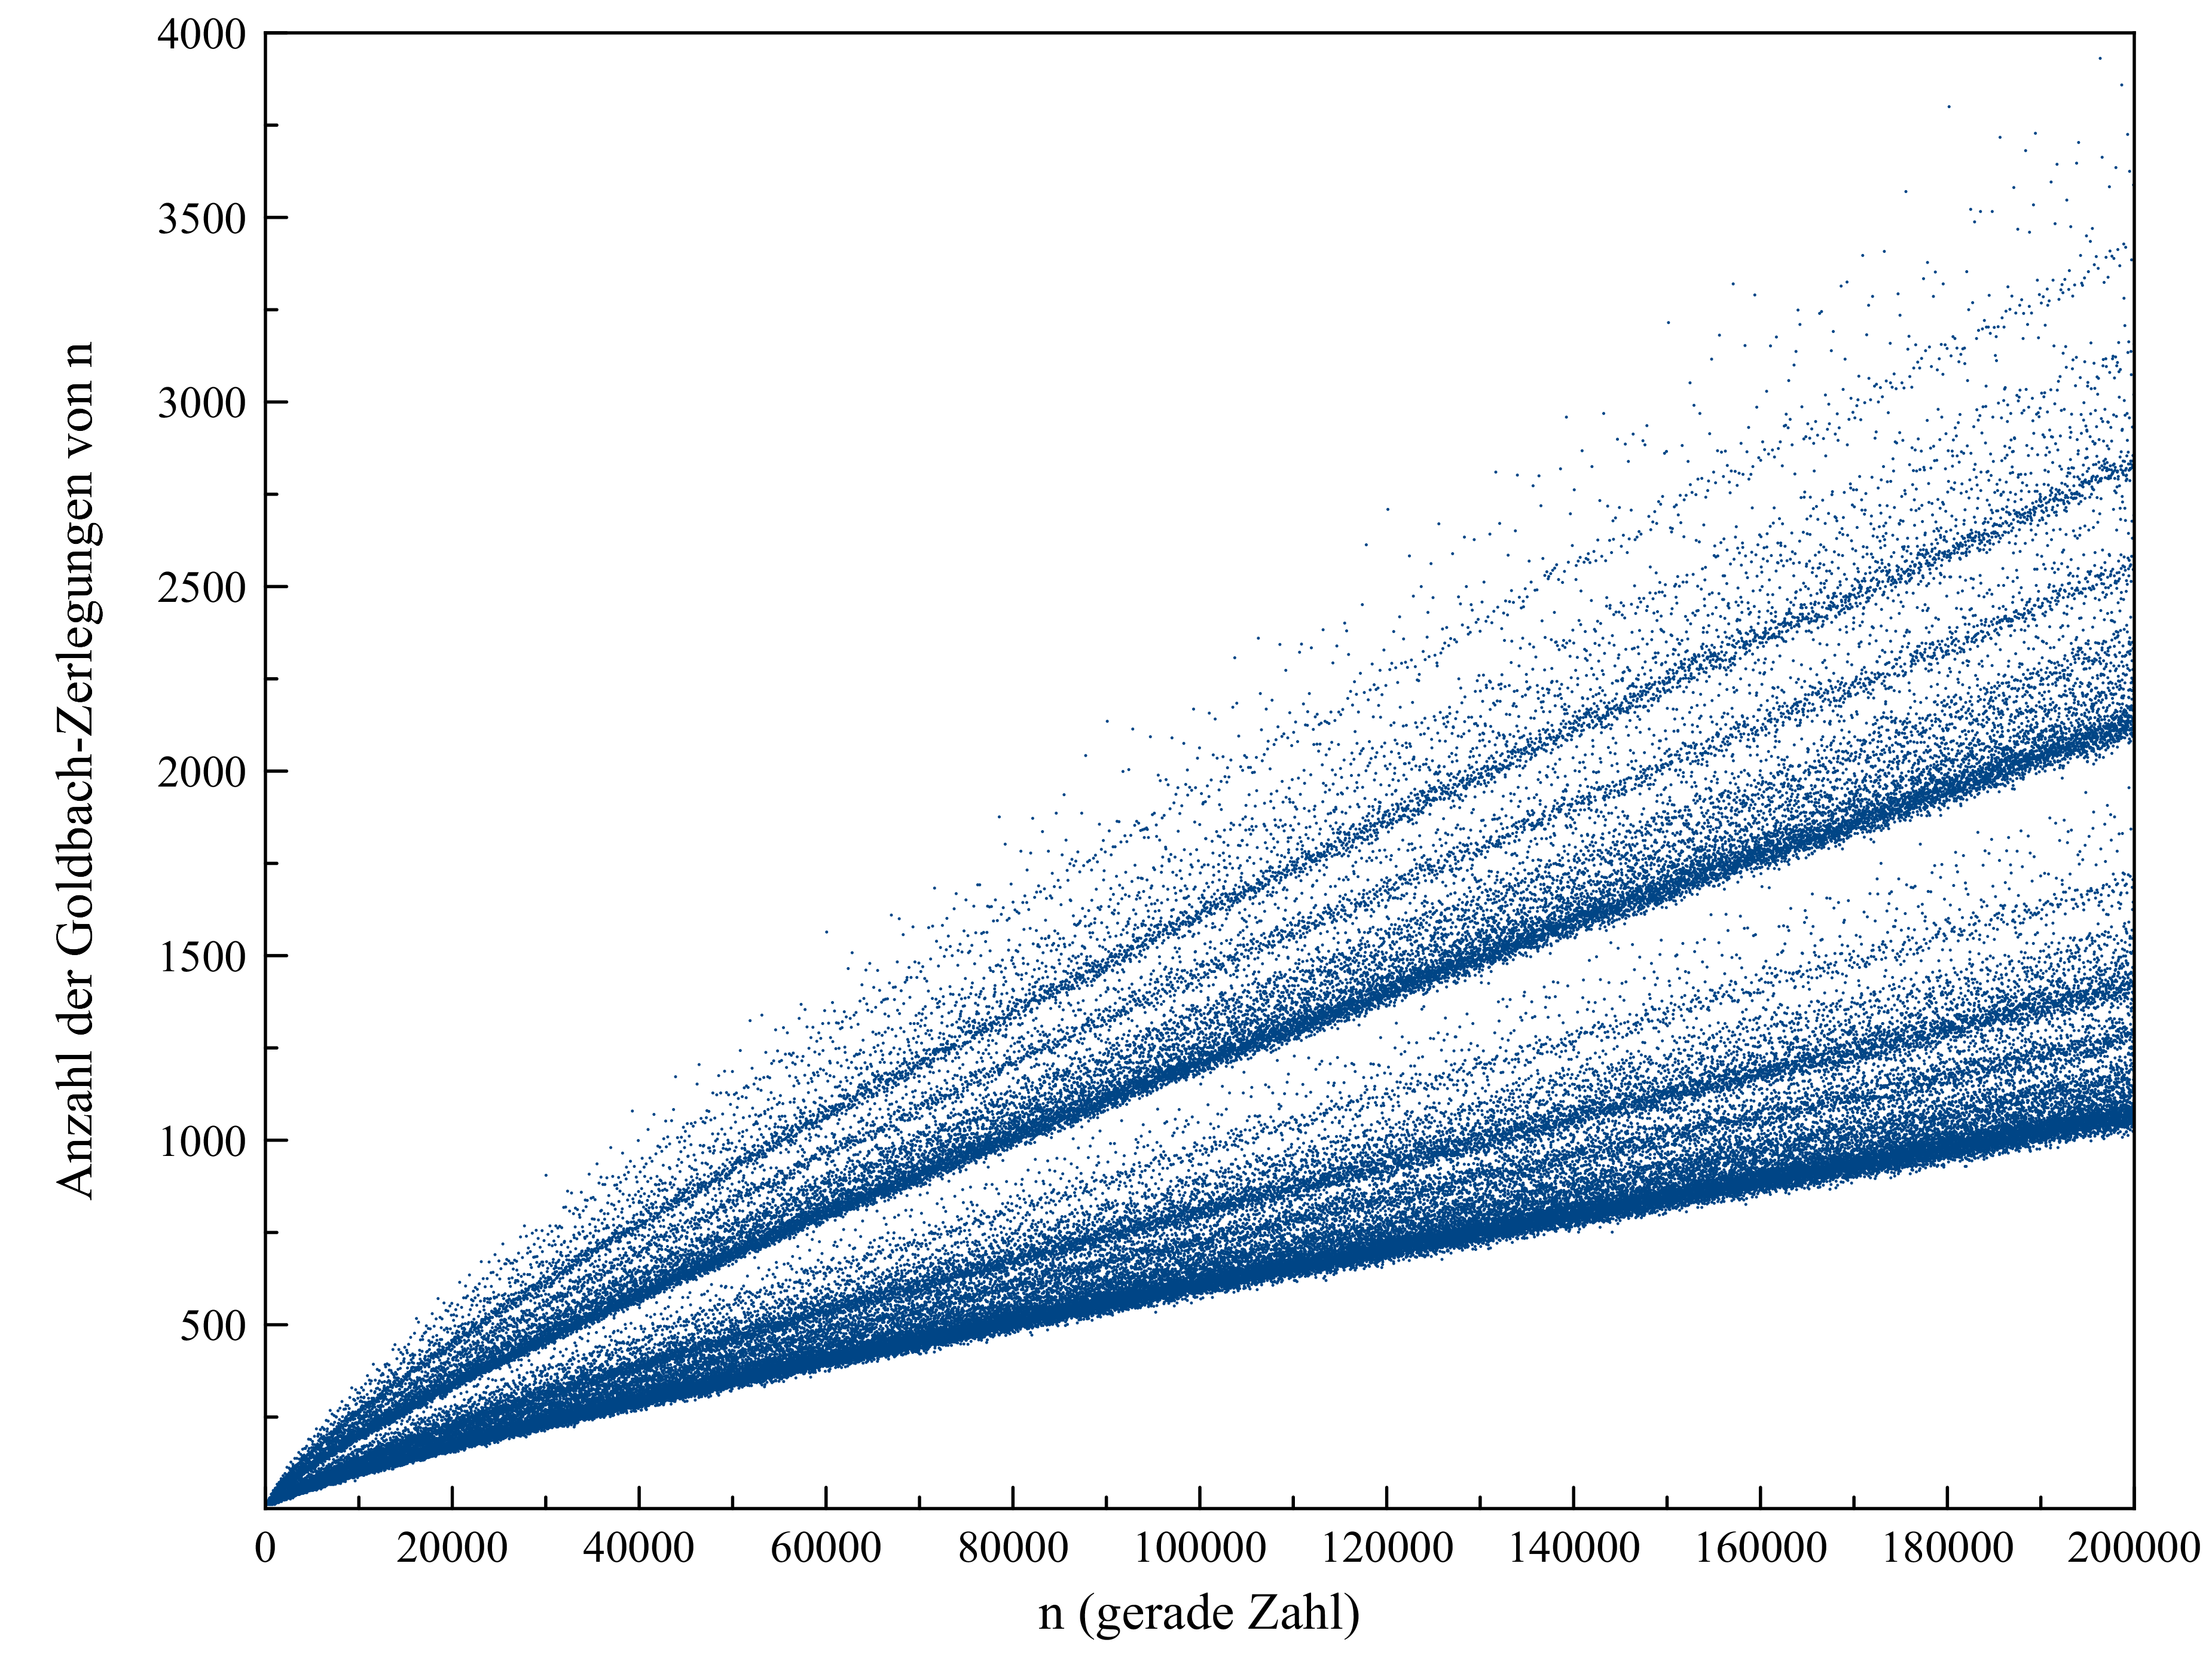
\includegraphics[width=0.8\linewidth]{img/Goldbach200000.png}
\caption{Anzahl der Moeglichkeiten gerade Zahlen nach Goldbach als Summe zweier Primzahlen darzustellen}
\label{fig:goldbach_diagramm}
\end{figure}
%\subsection{Programmbeispiel}
